\documentclass[conference]{IEEEtran}
\IEEEoverridecommandlockouts
\usepackage{cite}
\usepackage{amsmath,amssymb,amsfonts}
\usepackage{algorithmic}
\usepackage{graphicx}
\usepackage{textcomp}
\usepackage{listings}
\usepackage{graphicx}
\graphicspath{ {images/} }
\def\BibTeX{{\rm B\kern-.05em{\sc i\kern-.025em b}\kern-.08em
    T\kern-.1667em\lower.7ex\hbox{E}\kern-.125emX}}

\title{\#5 Assignment - Implementing Concurrency - CMPT 383}
\author{Luiz Fernando Peres de Oliveira - 301288301 - lperesde@sfu.ca}
\date{November 26th, 2017}
\begin{document}
\maketitle
\section{Introduction}
As mentioned on \textbf{Assignement \#4}, Numerical methods for scientific problems, especially in engineering and science, are frequently related to solving problems for large matrices (such as image processing). Traversing matrices, for example, is one of the heaviest numerical computations as, for a given matrix \textbf{m} with \textit{r} rows and \textit{c} columns, it has known time complexity of $O(r\times c)$. This is a very hard task to be accomplished by a computer when we have very large matrices to traverse, and, for this reason, one might take advantages of concurrent programming. The idea is deconstructing a problem in small pieces and solving them concurrently and only them assembling the small pieces in order to solve the whole problem (also known as \textbf{divide and conquer}).
\\\\
The work below will discuss and illustrate how efficiently different paradigms use matrices to solve a given problem. However, at this time we are merging the reasearch on libraries on \textbf{Assignments \#2} with the matrix operations (\textbf{Assignments \#4}).
\\\\
For this assignment will be using \textit{(Functional Programming: Haskell with \textit{Control.Concurrent module}, Object-oriented Programming: Java with \textit{Runnable interface}, Scripting Language: Python with \textit{threading}, and Procedural Programming: C with \textit{pthread library})}.
\\\\
Furthemore, it will be implemented, run (\textbf{concurrently}), evaluated and discussed the map functions \textbf{add}, \textbf{multiply} and \textbf{custom} for each paradigm/language/library described above. Each one of these map functions take a \textit{matrix} \textbf{m} as input and return a \textit{matrix} \textbf{m'} as output. They can be represented mathematically as:

\begin{itemize}
	\item \textbf{add}: $c_{ij} = a_{ij} + b_{ij}$
	\item \textbf{multiply}: $c_{ij} = a_{ik} \times b_{kj}$
	\item \textbf{custom}: $c_{ij} = max(a_{ij}, b_{ij}) + a_{ij}^2 + b_{ij}^2$
\end{itemize}

Finally, the map functions described above will be compared against a data $d$ starting from a matrix $m$ of size $10\times10$ and will then be increased of an order of magnitude $100\times100$ until we notice that the target code takes longer to execute. It is important to notice that this assignment will execute every single of the map functions described above \textit{concurrently}. At the end, every single paradigm will be evaluated. It is important to know that all map functions described above were already implemented on \textbf{Assignment \#4}.

\section{Related Work, Background and Applications}
There are numerous applications in which matrices are a useful for scientific programming. For instance, matrices are largely used in the field of linear systems as a mean to represent and manipulate finite dimensional vector spaces. Matrices are are also very important in the field of linear algebra which is one of the most crucial tools in math. Some real-world applications for matrices are:  

\begin{itemize}
	\item \textbf{Computer Graphics and Image Processing}: Your computer graphics are represented by matrices. The major task of the \textit{GPU} is to calculate more than a billion matrix operations per second. Also, reflection and distortion effects applied on images such as the Gaussian and Sobel operators are represented by matrices as well as the images themselves.
	\item \textbf{Linear systems arithmetic}: Linear systems take advantage of matrix arithmetic. For instance, error-correcting codes and linear differential equations.
	\item \textbf{Supports Graph Theory}: Graphs may be abstracted as matrices.
	\item \textbf{Probability and Statistics}: The field of probability and statistics use matrix representations such as probability vectors of a neural system and Markov Chains on stochastic matrices.
	\item \textbf{2D and 3D Geometry}: Matrices 
\end{itemize}

\section{Implementation}

\textbf{ Object-oriented Programming - Java }\\
The way Object-oriented programming paradigm behaves regarding scientific programming (together with concurrency) can be related to the Object-oriented language we are using, because such paradigm is often implemented in multi-paradigm languages. For example, \textit{Java, Objective-C and Pony} will most likely have different ways and use different methods for processing numerical computations and concurrency, in spite of being object-oriented languages.
\\\\
In Java, we implement the \textit{Runnable} interface or extend the class \textit{Thread} if you want your code to be divided in multiple threads, allowing multitasking and consequently concurrency. Having a \textbf{Thread} class that implements \textit{Runnable}, you must implement a method named $run()$ (defined by the \textit{Runnable} interface). This method is called when your \textbf{thread object} is $started$.
\\\\
On the code below, you will see how one would represent the map functions concurrently \textbf{add}, \textbf{multiply} and \textbf{custom} in Java.
\\
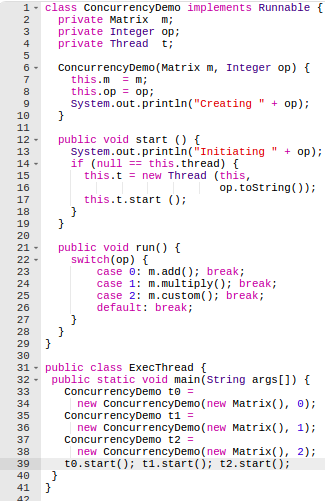
\includegraphics[scale=0.6]{java_code_5}

The previous Java code is expected to traverse matrices as fast as C (as already compared on \textbf{Assignment \#4}) and in fact (with limitations on the JVM), it is very hard to distinguish the differences between that code and a given C code for the same task. You can of course see that the Java code is very verbose regarding such simple functions. In this way, our class will be instantiated into an object of type \textbf{Matrix} and only them, after setting it up properly, we would be able to use all the power of this language. Also, this Java code allows us to use custom sizes for our data $d$ described on the introduction of this work. 

\textbf{ Scripting Language - Python }
As said (and proved) on previous assignments, scripting languages usually run slower than compiled languages (because of the time that is spent on just-in-time translations). Python has a slight advantage on other scripting languages because it uses many libraries written in pure C, boosting the process of interpreting programs.
\\\\
\textit{Python} has a number of different concurrency \textbf{constructs} such as \textit{threading}, \textit{queues} and \textit{multiprocessing}. The \textit{threading} module used to be the primary way of accomplishing concurrency. Python is also largely used and you can find many open source libraries over the internet related to concurrent programming, once it requires a lot of legwork in order to implement (and understand) it, if you compare with languages prepared for that, such as \textit{Erlang}.
\\\\
Compared to other languages, Python is the one of the ones with clearest code and helps us understand why the scientific community enforce the use of this tool. The code below represents how one would implement the map functions \textbf{add}, \textbf{multiply} and \textbf{custom} concurrently in Python.

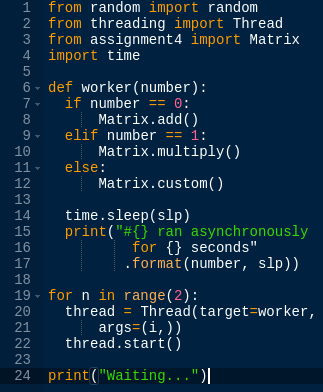
\includegraphics[scale=0.7]{python_code_5}

\textbf{ Procedural Programming - C }

Procedural programming, as its name suggests, bases itself in procedure, functions or sub-routines calls (not to be confused with mathematical functions related to functional programming). It also follows the imperative paradigm as it makes explicit reference to changing-state, performs a series of well-structured sequential steps and may have side effects. Systematically, it embraces a succession of statements and functions to perform a computational task or program. Pascal, C and Go are example of procedural languages.
\\One must link the $pthread$ library in order to use most(if not all) of multithreading capabilities in \textbf{C}. There are a few particularities for that, such as declaring a variable (let us call it $tid$ or $pid$), with type of $pthread\_t$, which is type representing the id of a thread based on an integer (which is the same as explained on \textit{Erlang} for $pid$), used to retrieve and handle the thread in the system.
\\\\
On the code below, you will see how one would represent the map functions \textbf{add}, \textbf{multiply} and \textbf{custom} concurrently in C.

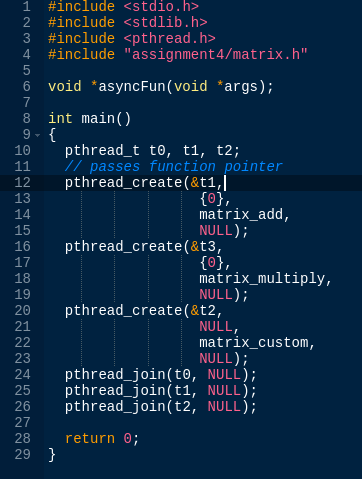
\includegraphics[scale=0.62]{c_code_5}

\textbf{ Functional Programming - Haskell }

Functional programming in general appears to have many beautiful ways of traversing matrices, given (in theory) the lack of side effects and its foundation of applying mathematical functions to the real world, however, in practice, this may not work as beautiful as it seems because a bigger problem may be divided into many small problems (function calls, as high order functions are always broken down in other smaller functions), which may impact on the speed of a given program, once that it would be faster if the process was done linearly$[5]$ (the way that imperative languages would try to solve this category of problems). Haskell will be the representative of the Functional Programming paradigm for this assignment.
\\\\
Haskell provides a mechanism to allow the user to control the of concurrency by indicating what computations may be done. To use the power of concurrency one must use the $Control.Concurrent$ module. For that, the use of $MVars$ is very important once they do the managing concurrent access to shared resources, and communicating across threads. See the code below:
\\\\
On the code below, you will see how one would represent the map functions \textbf{add}, \textbf{multiply} and \textbf{custom} concurrently in Haskell.

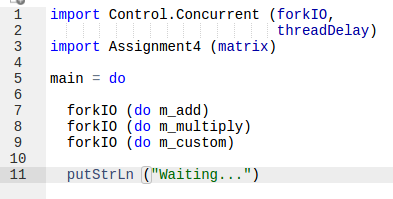
\includegraphics[scale=0.60]{haskell_code_5}

\section{Evaluation Environment}
Macbook Pro:\\
- 2.2GHz quad-core Intel Core i7 processor\\
- 16GB RAM

\section{Results}

The results below represent the time execution for the languages here compared. Important to notice that the code snippets above were reduced and the full implementation can be seen on \textbf{Assignment \#4}. The evaluation was on done a \textbf{sparsed} and \textbf{dense} matrices \textbf{m} and data $d$.

\begin{itemize}
\item $10\times10$
\item $100\times100$
\item $1000\times1000$
\item $10000\times10000$
\item $100000\times100000$
\end{itemize} 

The time execution is as described on the Graph below:

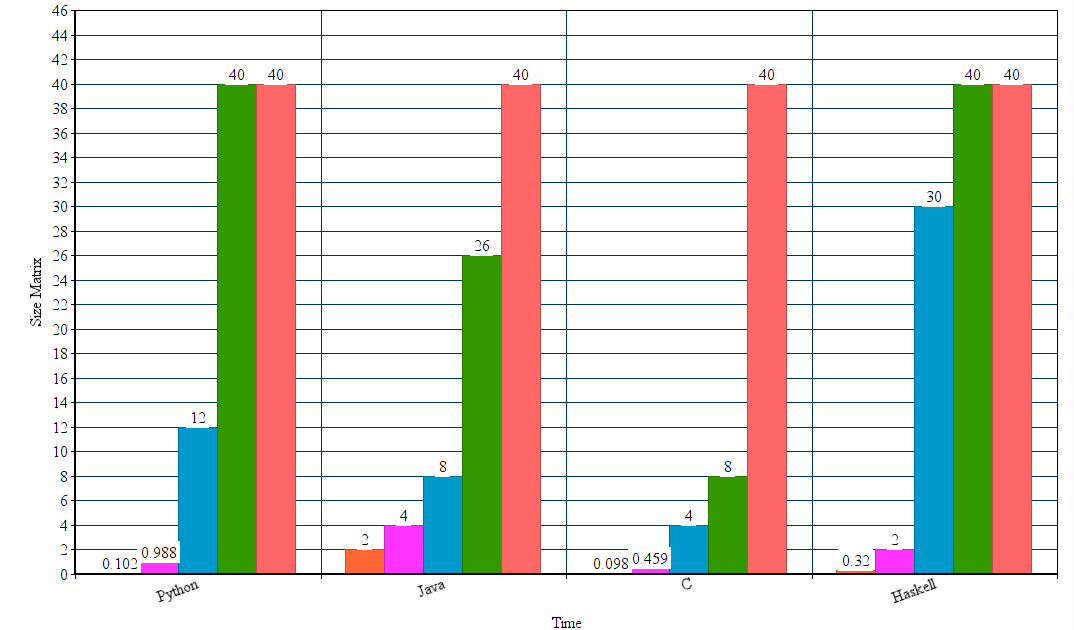
\includegraphics[scale=0.25]{graph_codes}

\small{\textit{* The number \textbf{40} represents a long time (or infinite) to execute a task. 
We can see that the smaller the bar, the faster the language is. On the discussion section will be given details about the time execution of each language/paradigm. We will also compare it with \textbf{Assignment \#4} }}

\section{Discussion}
After evaluating all languages on this assignment, \textbf{C}, and \textbf{Java} have (again) better performance than \textbf{Haskell} and \textbf{Python}. Compared with \textbf{Assignment \#4}, however, all of the languages have improved a lot, running at least at half the speed of the same languages on \textbf{Assignment \#4}. Concurrency boosted all languages because it was possible to run many tasks at same time and it would completely used the different processor cores.
\\\\
Again, because \textit{C} and \textit{Java} are imperative programming languages, and both are compiled (except that Java is compiled to bytecode and them interpreted by the JVM), they are able to perform fast scientific computations, whereas \textit{Haskell} will be constrained by the functional programming paradigm and \textit{Python} is a Scripting Language.
\\\\
With \textbf{Assignment \#4}, we had a hint of which languages would be in the top of \textbf{Assignment \#5} and the results were very alike, in spite of a general improvement on the speed of them.
\\\\
At this time, Python was not the slowest language and did not complete all tests (only around 60\% of the benchmarks). Haskell did not improve a lot, as I was expecting it to be. This seemed to happen because its compiler tries to make it as fast as it could. The improvements for scientific computing on Haskell was around $20\sim30\%$. All the other languages improved at least $40\%$.
\\\\
Regarding \textit{Java}, the \textit{JVM} warm up gave a huge boost to the execution of the scientific computations here evaluated.
\\\\
To conclude, the rank of languages ended up with:
\\\\
- \textbf{1st place: C}\\
\textit{C} is evaluated as the best one (in comparison with the other ones in this assignment) because of its native advantages over the other languages. C is also one of the oldest languages amongst this set as has proven that it is indeed very optimized.
\\\\
- \textbf{2nd place: Java}\\
The \textit{JVM} is slow, but not so slow. There still some advantage because of its \textit{JVM's} warm-up. Some people say that scientific programming in Java is actually possible and there are a lot of support for it on its community, which was proved in this assignment.
\\\\
- \textbf{3rd place: Python}\\
Although it has many libraries written in C, having advantage over other languages, it did not help the execution of the program.
\\\\
- \textbf{4th place: Haskell}\\
I also believe strongly that \textit{Haskell} will took the last position because of the reasons discussed before on this assignment.
\begin{thebibliography}{00}
\bibitem{b1} "Erlang -- Concurrent Programming", Erlang.org, 2017. [Online]. Available: http://erlang.org/doc/getting\_started/conc\_prog.html. [Accessed: 09- Oct- 2017].

\bibitem{b2} "The Hitchhiker's Guide to Concurrency | Learn You Some Erlang for Great Good!", Learnyousomeerlang.com, 2017. [Online]. Available: http://learnyousomeerlang.com/the-hitchhikers-guide-to-concurrency. [Accessed: 09- Oct- 2017].

\bibitem{b3} A. Miller, "Understanding actor concurrency, Part 1: Actors in Erlang", JavaWorld, 2017. [Online]. Available: https://www.javaworld.com/article/2077999/java-concurrency/understanding-actor-concurrency--part-1--actors-in-erlang.html. [Accessed: 09- Oct- 2017].

\bibitem{b4} "Concurrency - HaskellWiki", Wiki.haskell.org, 2017. [Online]. Available: https://wiki.haskell.org/Concurrency. [Accessed: 09- Oct- 2017].

\bibitem{b5} "7.26.�Concurrent and Parallel Haskell", Downloads.haskell.org, 2017. [Online]. Available: https://downloads.haskell.org/~ghc/7.8.4/docs/html/users\_guide/lang-parallel.html. [Accessed: 09- Oct- 2017].

\bibitem{b6} "Haskell/Concurrency - Wikibooks, open books for an open world", En.wikibooks.org, 2017. [Online]. Available: https://en.wikibooks.org/wiki/Haskell/Concurrency. [Accessed: 09- Oct- 2017].

\bibitem{b7} "Lesson: Concurrency (The Java™ Tutorials > Essential Classes)", Docs.oracle.com, 2017. [Online]. Available: https://docs.oracle.com/javase/tutorial/essential/concurrency/. [Accessed: 09- Oct- 2017].

\bibitem{b8} 2. Lars Vogel (c) 2009, "Java concurrency (multi-threading) - Tutorial", Vogella.com, 2017. [Online]. Available: http://www.vogella.com/tutorials/JavaConcurrency/article.html. [Accessed: 09- Oct- 2017].

\bibitem{b9} "Python Multithreading Tutorial: Concurrency and Parallelism", Toptal Engineering Blog, 2017. [Online]. Available: https://www.toptal.com/python/beginners-guide-to-concurrency-and-parallelism-in-python. [Accessed: 09- Oct- 2017].

\bibitem{b10} "17. Concurrent Execution — Python 3.6.3 documentation", Docs.python.org, 2017. [Online]. Available: https://docs.python.org/3/library/concurrency.html. [Accessed: 09- Oct- 2017].

\bibitem{b11} C. Threads, "Concurrency in Threads", Stackoverflow.com, 2017. [Online]. Available: https://stackoverflow.com/questions/7978152/concurrency-in-threads?rq=1. [Accessed: 09- Oct- 2017].

\bibitem{b12} "Go-style concurrency in C | Hacker News", News.ycombinator.com, 2017. [Online]. Available: https://news.ycombinator.com/item?id=10585505. [Accessed: 09- Oct- 2017].

\bibitem{b13} 2017. [Online]. Available: https://gcc.gnu.org/wiki/cauldron2015?
action=AttachFile\&do=get\&target=Torvald+Riegel
\_+Modern+concurrent+code+in+C.pdf. [Accessed: 09- Oct- 2017].

\bibitem{b14} "Freund\_HLA", 2017. [Online]. Available: https://www.math.ucdavis.edu/~freund/freund\_HLA.pdf. [Accessed: 28- Oct- 2017].

\bibitem{b15} "Big O notation", En.wikipedia.org, 2017. [Online]. Available: https://en.wikipedia.org/wiki/Big\_O\_notation. [Accessed: 28- Oct- 2017].

\bibitem{b16} "Tweag I/O - Enter the matrix, Haskell style", Tweag.io, 2017. [Online]. Available: https://www.tweag.io/posts/2017-08-31-hmatrix.html. [Accessed: 28- Oct- 2017].

\bibitem{b17} "Functional vs. Imperative Programming", Ryanhmckenna.com, 2017. [Online]. Available: http://www.ryanhmckenna.com/2014/11/functional-vs-imperative-programming.html. [Accessed: 28- Oct- 2017].

\bibitem{b18} "hmatrix", 2017. [Online]. Available: http://dis.um.es/~alberto/material/hmatrix.pdf. [Accessed: 28- Oct- 2017].

\bibitem{b19} "For scientific computing, is Java useful in a way that C or Python aren't? - Quora", Quora.com, 2017. [Online]. Available: https://www.quora.com/For-scientific-computing-is-Java-useful-in-a-way-that-C-or-Python-arent. [Accessed: 28- Oct- 2017].

\bibitem{b20} "Scientific Computation", Introcs.cs.princeton.edu, 2017. [Online]. Available: https://introcs.cs.princeton.edu/java/90scientific/. [Accessed: 28- Oct- 2017].

\bibitem{b21} "Java And Cpp Platforms For Scientific Computing", 2017. [Online]. Available: https://inside.mines.edu/~dhale/papers/Hale06JavaAndCppPlatformsForScientificComputing.pdf. [Accessed: 28- Oct- 2017].

\bibitem{b2} P. Knoll and S. Mirzaei, "Scientific computing with Java", 2017.

\end{thebibliography}
\end{document}